\section{Results}
\label{sec:results}

One finding, two regimes. The rest of this section is the BFCL split
tests (Section~\ref{sec:results:regime}), the distractor probe with
the target removed (Section~\ref{sec:results:probe}), the Qwen3
size-axis curve along with the way the per-arm peak shifts as scale
grows (Section~\ref{sec:results:scaling}), per-tier RVR validation
(Section~\ref{sec:results:rvr}), and the trace pass we read as the
most plausible account of the Anthropic null
(Section~\ref{sec:results:trace-inspection}).

% =========================================================================
\subsection{Regime tests: TFR is at or near zero across BFCL multi-turn splits}
\label{sec:results:regime}
% =========================================================================

Per-call TFR for Sonnet~4.6 and Haiku~4.5 across the three BFCL
multi-turn splits under $\mathrm{C}_0$ is in Table~\ref{tab:regime}.
Every cell in the regime grid is $\boldsymbol{0/N}$ (C0 calls only).
Clopper--Pearson $95\%$ per-cell upper bound is $\leq\!3.63\%$;
pooled over the $661$ C0 regime calls, $\leq\!0.45\%$.

\begin{table}[t]
\caption{Regime-test TFR by model and BFCL split under $\mathrm{C}_0$.
Cells are events / parsed calls.}
\label{tab:regime}
\centering
\small
\setlength{\tabcolsep}{8pt}
\begin{tabular}{lccc}
\toprule
Model & base & miss\_func & long\_ctx \\
\midrule
Sonnet 4.6 & 0/116 & 0/128 & 0/81 \\
Haiku 4.5  & 0/109 & 0/120 & 0/107 \\
\bottomrule
\end{tabular}
\end{table}

BFCL designed the \texttt{miss\_func} split to elicit fabrication by
removing a needed function. Both Anthropic models route around the
missing tool by chaining smaller calls instead (one trace in
Section~\ref{sec:results:trace-inspection}). Qwen3-8B does not behave
the same way. % NUMBERS_TODO: Qwen3-8B miss_func cell (claimed 5/258=1.94%) absent from aggregator; rerun and reconcile against the base full-probe 9/615=1.46%.
On the same split it logs $5/258 = 1.94\%$, slightly
above the $1.46\%$ on the aligned \texttt{multi\_turn\_base} split.
That is what BFCL's design predicts when the registry is deliberately
incomplete.

% =========================================================================
\subsection{Anthropic stability check across $5$ model versions}
\label{sec:results:probe}
% =========================================================================

The probe injects one synthetic distractor tool into a registry from
which the real \emph{target} tool has been removed. This is a
Czapla-style scenario: the agent expects a tool to exist, and the
registry offers only a similarly-named distractor. Four distractor
types (near-name, synonym, matched-random, unrelated) are tested on
$N\!=\!15$ \texttt{multi\_turn\_base} tasks where $\mathrm{C}_0$
already passes without modification.

We tested five Anthropic 4.x versions over an $11$-month window
across the Opus, Sonnet, and Haiku families. On this probe every cell
is $\boldsymbol{0/N}$ (Table~\ref{tab:anth-temporal};
$95\%$ pooled upper bound $\leq\!0.16\%$). Combine the regime cells
with the probe cells and the $\mathrm{C}_0$ Anthropic audit pools to
\textbf{$\boldsymbol{0/2{,}599}$} (per-call aggregator, deduplicated
across overlapping run-ids), or $\leq\!0.115\%$.

\begin{table}[t]
\caption{Anthropic 4.x distractor probe with target removed ($\mathrm{C}_0$).
Pooled $\mathrm{C}_0$ over regime $+$ probe is $0/2{,}599$,
$\leq\!0.115\%$; the $\mathrm{C}_1$ subset adds $0/678$ at
$\leq\!0.441\%$.}
\label{tab:anth-temporal}
\centering
\small
\setlength{\tabcolsep}{6pt}
\begin{tabular}{lrc}
\toprule
Model & $N$ & TFR \\
\midrule
Opus 4.7        & 293   & 0 \\
Sonnet 4.6      & 561   & 0 \\
Sonnet 4.5      & 285   & 0 \\
Sonnet 4        & 253   & 0 \\
Haiku 4.5       & 525   & 0 \\
\midrule
Pooled probe & \textbf{1{,}917} & \textbf{0} \\
\bottomrule
\end{tabular}
\end{table}

On this benchmark, Anthropic models do not invent tool names. Five
versions, eleven months, the same null. We can think of two readings
that fit the data and we cannot separate them. One is that
post-training has been hardened against fabrication. The other is
that BFCL's redundant tool basket lets the agent route around a
missing tool rather than guess at one. Honestly, both probably help
in different proportions. The gap with prior work is less mysterious
once you remember that older models had no tool-use post-training
and that prior benchmarks aggregated per task rather than per call.

% =========================================================================
\subsection{Qwen3 scaling curve: TFR is non-monotonic across $0.6$B--$32$B}
\label{sec:results:scaling}
% =========================================================================

The $14$B$\to\!32$B drop, $1.87\%$ to $0\%$, is our central
intra-family result. The $32$B model produces no fabrications under
our probe ($N\!=\!224$, CP $95\%$ upper bound $\leq\!1.33\%$). That
upper bound is wide enough to overlap the $14$B point estimate, so
``collapse'' here should be read as ``not-detected at this $N$,'' not
as emergent capability. Figure~\ref{fig:scaling} and
Table~\ref{tab:qwen3-scale} show the pattern. Pooled per-call TFR
rises from $0\%$ ($0/75$, $\leq\!3.92\%$) at $0.6$B, peaks at $14$B
($5/268=1.87\%$), and then collapses back to $0\%$ ($0/224$,
$\leq\!1.33\%$) at $32$B. The per-arm peak shifts across sizes. $1.7$B peaks on
\emph{near\_name} ($2/54=3.7\%$). $4$B peaks on
\emph{matched\_random} ($3/56=5.4\%$). $8$B peaks on
\emph{matched\_random} again ($3/129=2.3\%$). $14$B peaks on
\emph{synonym} ($5/69=7.2\%$).

\begin{figure}[t]
\centering
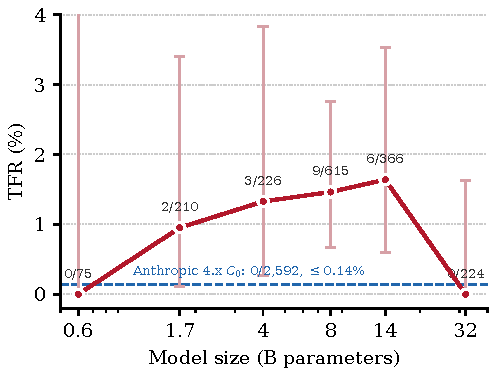
\includegraphics[width=0.9\linewidth]{figures/fig1_scaling_curve}
\caption{Qwen3 family TFR scaling curve, opaque baseline
$\mathrm{C}_0$, four-distractor probe with target removed. Error bars
are Clopper--Pearson 95\% CIs. Anthropic 4.x upper bound (dashed blue)
includes all $5$ tested versions over $11$ months. The intra-family
non-monotone shape and the persistent gap between the open-source
$\sim\!2{-}14\,$B band and the Anthropic upper bound is the
paper's headline.}
\label{fig:scaling}
\end{figure}

\begin{table}[t]
\caption{Qwen3 scaling curve under $\mathrm{C}_0$ (target removed).
Cells are events / parsed calls; bold marks the per-row peak.}
\label{tab:qwen3-scale}
\centering
\small
\setlength{\tabcolsep}{4pt}
\begin{tabular}{lccccr}
\toprule
Size & near & syn. & match. & unrel. & Pooled \\
\midrule
0.6B  & 0/18 & 0/20 & 0/18 & 0/19 & 0/75 \\
1.7B  & \textbf{2/54} & 0/54 & 0/49 & 0/53 & 2/210 \\
4B    & 0/57 & 0/54 & \textbf{3/56} & 0/59 & 3/226 \\
8B    & 1/219 & 3/134 & \textbf{3/129} & 2/133 & 9/615 \\
14B   & 0/63 & \textbf{5/69} & 0/67 & 0/69 & 5/268 \\
32B   & 0/55 & 0/57 & 0/55 & 0/57 & 0/224 \\
\bottomrule
\end{tabular}
\end{table}

A same-family check from the previous Qwen generation strengthens
the picture. Qwen2.5-7B-Instruct on the same probe gives
$28/459 = 6.10\%$, higher than any Qwen3 size at any arm. This is
not an apples-to-apples generation comparison. Qwen2.5 has different
post-training and a different tokenizer. But it does say the
non-monotone shape we report is not a Qwen3-specific artefact of one
release. The lineage carries the failure mode.

Commercial models track the Anthropic null rather than the Qwen3
band. On the same probe, the OpenAI gpt-4.1 and gpt-4o tiers also log
$0\%$ TFR --- gpt-4.1 $0/404$, gpt-4.1-mini $0/408$, gpt-4.1-nano
$0/409$, gpt-4o $0/419$, gpt-4o-mini $0/430$ (per-model Clopper--Pearson
$95\%$ upper bounds $\leq\!0.69$--$0.74\%$), pooling to $0/2{,}070$ at
$\leq\!0.14\%$. The open-vs-closed split is the cross-vendor pattern:
zero-event commercial frontiers on one side, the Qwen-family
$0.95$--$1.87\%$ band on the other.

We treat the shape itself as the result. Most readers would guess
that $14$B fabricates less than $1.7$B. It does not. We read the
traces as suggesting why. At $1.7$B the model rarely emits
well-formed tool calls, leaving little surface to fabricate on.
At $14$B it formats calls fluently but does not check the registry.
At $32$B it does both. The peak distractor type also moves with
scale: $1.7$B is most often fooled by a near-name twin, $4$B and
$8$B by a length-and-arity-matched random tool, and $14$B by a
synonym. Six points do not support a fitted scaling law. The
shape is consistent though. At each scale the dominant failure is
whichever distractor that scale is best primed to mimic.

% =========================================================================
\subsection{RVR per-tier validation: $14 \to 0$ events across the Qwen3 sweep}
\label{sec:results:rvr}
% =========================================================================

We applied the registry-visible re-prompt $\mathrm{C}_1$ on the four
Qwen3 sizes that produced $\mathrm{TFR}\!>\!0$ in $\mathrm{C}_0$.
Across $\sim\!944$ matched calls in $\mathrm{C}_1$, RVR prevents
$\boldsymbol{14}$ of $\boldsymbol{14}$ hallucination events. Zero
remain. Per-tier prevention is in Table~\ref{tab:rvr-validation}.

\begin{table}[t]
\caption{RVR per-tier validation on Qwen3 sizes with non-zero $\mathrm{C}_0$
events. Cells are events / parsed calls. These are the paired
$\mathrm{C}_0$/$\mathrm{C}_1$ matched-run subset used for the
prevention contrast; the $\mathrm{C}_0$ denominators here (e.g.\ 8B
$4/269$) are the matched-run cells and are smaller than the full
distractor-probe pool reported in Table~\ref{tab:qwen3-scale} (8B
$9/615$), which aggregates all probe runs at that tier.}
\label{tab:rvr-validation}
\centering
\small
\setlength{\tabcolsep}{8pt}
\begin{tabular}{lccc}
\toprule
Tier & $\mathrm{C}_0$ & $\mathrm{C}_1$ & Prevented \\
\midrule
Qwen3-1.7B & 2/210 & 0/200 & 2/2 \\
Qwen3-4B   & 3/226 & 0/228 & 3/3 \\
Qwen3-8B   & 4/269 & 0/258 & 4/4 \\
Qwen3-14B  & 5/268 & 0/259 & 5/5 \\
\midrule
Pooled     & \textbf{14/973} & \textbf{0/945} & \textbf{14/14} \\
\bottomrule
\end{tabular}
\end{table}

The Anthropic $\mathrm{C}_1$ probe (Sonnet~4.6 + Haiku~4.5)
preserves $0/539$ hallucinations. The strict-pass subset drops:
Sonnet $60/60\!\to\!53/60$ ($-11.7\,$pp), Haiku $60/60\!\to\!56/60$
($-6.7\,$pp). A Newcombe-hybrid TOST at the $5\,$pp margin gives
$p_{\mathrm{TOST}}\!=\!0.91$ (Sonnet) and $0.63$ (Haiku). At $N=60$
the test is underpowered ($1\!-\!\beta\!<\!0.30$), so we can call
neither non-inferiority nor inferiority. RVR stays zero-event on the
Anthropic frontier; the strict-pass cost is undetermined at this
$N$ (Section~\ref{sec:limitations:rvr-null}).

\begin{figure}[t]
\centering
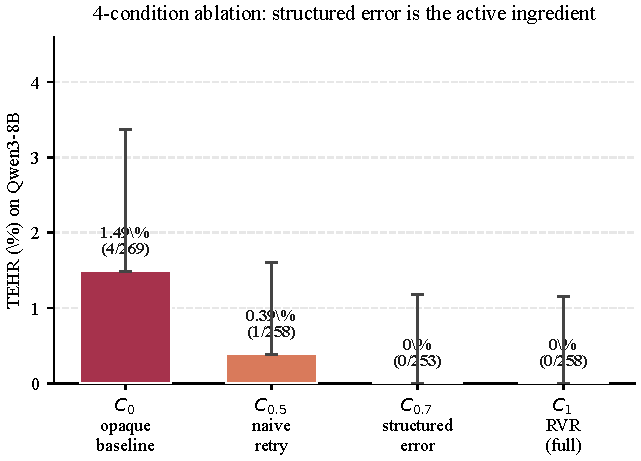
\includegraphics[width=0.95\linewidth]{figures/fig2_ablation_ladder}
\caption{Qwen3-8B 4-condition ablation. The structured-error
envelope ($\mathrm{C}_{0.7}$) drives the prevention; adding the
registry list ($\mathrm{C}_1$) yields no further reduction.}
\label{fig:ablation}
\end{figure}

The four-condition ladder on Qwen3-8B walks down a clean gradient.
Opaque baseline: $1.46\%$ ($9/615$, full probe). Naive retry: $0.39\%$
($1/258$). Structured envelope ($\mathrm{C}_{0.7}$): $0/448$
($\leq\!0.67\%$). Full RVR re-prompt ($\mathrm{C}_1$): $0/258$
($\leq\!1.15\%$). See
Figure~\ref{fig:ablation}. The structured envelope drives the
prevention. The registry list does not add anything detectable on
this tier. $\mathrm{C}_{0.7}$ already reaches zero, and stacking the
registry list on top buys no further prevention (Newcombe-hybrid
95\% CI on the $\mathrm{C}_1\!-\!\mathrm{C}_{0.7}$ difference:
$[-1.5, +1.4]$~pp). We read this as the message-level signal that
the previous call was rejected carrying the effect; the registry
content that follows is decorative on this tier. The practical
upshot is that a deployer who wants prevention without echoing
internal tool names can ship $\mathrm{C}_{0.7}$ and lose nothing.

\paragraph{Fisher's exact on the pooled $\mathrm{TFR}\!>\!0$
subset.} The $\mathrm{C}_0$/$\mathrm{C}_1$ denominators differ per
tier, so the trials are not paired at the call level; we treat the
four tiers as independent strata. We report \textbf{Fisher's exact
one-sided test} on the pooled $14/973$ vs.\ $0/945$ contingency:
$\mathbf{p = 7.1\!\times\!10^{-5}}$. Per-tier Fisher's exact
one-sided $p$ values are $\{0.24, 0.12, 0.058, 0.032\}$ for
$1.7$B/$4$B/$8$B/$14$B respectively. Each tier is individually
underpowered, but the sign is consistent. The pooled contrast
survives Holm--Bonferroni at
$p_{\mathrm{Holm}}\!=\!2.14\!\times\!10^{-4}$.

\paragraph{Trace inspection.}
\label{sec:results:trace-inspection}
On \texttt{multi\_turn\_miss\_func\_24} the Anthropic agent chains
five in-registry calls
(\texttt{pwd}$\!\to\!$\texttt{ls}$\!\to\!$\texttt{cd}$\!\to\!$\texttt{mkdir}$\!\to\!$\texttt{mv})
where a one-shot \texttt{mv\_recursive()} would have been
fabricated. We inspected $30$ near-name probe traces. Agents reach
for other in-registry tools (\texttt{find}, \texttt{cd},
\texttt{diff}, \texttt{echo}, \texttt{touch}) rather than the
removed target's or the distractor's name. Cost: Anthropic audit
\$$73$; Qwen3 sweep \$$0$ marginal on M5/32GB. RVR adds zero
provider round-trips on hits, one on misses; the rendered registry
is $\sim$100--200 tokens at $\leq$25 tools (under 5\% of context).
